\documentclass[12pt,a4paper]{scrartcl}
\usepackage{amsmath}
\usepackage{amsfonts}
\usepackage{amsthm}
\usepackage{amssymb}
\usepackage[latin1]{inputenc}
\usepackage{mathptmx}
\usepackage{}
\usepackage{array}
\usepackage{color}
\usepackage{hyperref}
\usepackage{url}
\usepackage{graphicx}
\usepackage{multicol}
\usepackage{dsfont}

\usepackage{booktabs}

%\usepackage[ignoreunlbld,nomsgs]{refcheck}

\usepackage{pgf, tikz}
\usepackage{color}

% !TeX spellcheck = en_US

%\textwidth=15cm \textheight=22cm \topmargin=0.5cm
%\oddsidemargin=0.5cm \evensidemargin=0.5cm

\usepackage[T1]{fontenc}

\usepackage[scaled=0.8]{beramono}

\usepackage{fancyvrb} \RecustomVerbatimEnvironment{Verbatim}{Verbatim}
{xleftmargin=15pt, frame=single, fontsize=\small}

\begin{document}
	
\thispagestyle{empty}
	

\begin{center}
	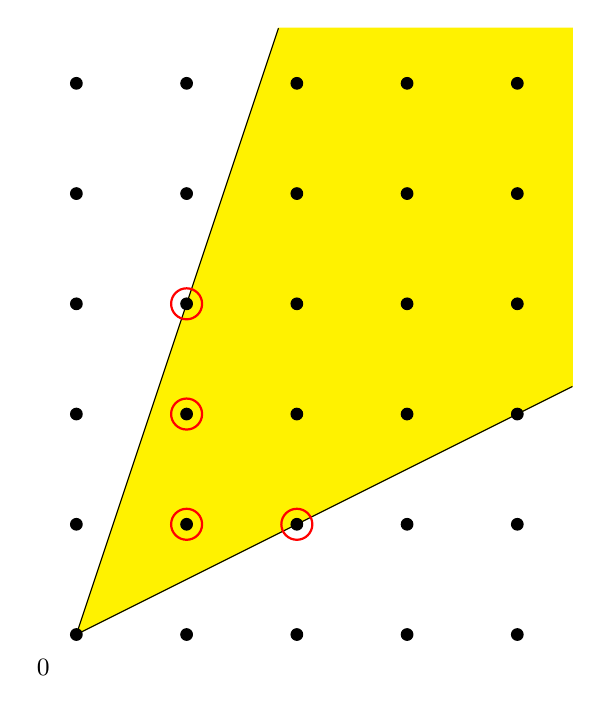
\begin{tikzpicture}[scale=1.4]
	\filldraw[yellow] (0,0) -- (1.833,5.5) -- (4.5,5.5) -- (4.5,2.25) -- cycle;
	\draw (0,0) -- (1.833,5.5);
	\draw (0,0) -- (4.5,2.25) node at (-0.3,-0.3){\small $0$};
	\foreach \x in {0,...,4}
	\foreach \y in {0,...,5}
	{
		\filldraw[fill=black] (\x,\y)  circle (1.5pt);
	}
	\draw[red,thick] (1,1) circle (4pt);
	\draw[red,thick] (1,2) circle (4pt);
	\draw[red,thick] (1,3) circle (4pt);
	\draw[red,thick] (2,1) circle (4pt);
	\end{tikzpicture}
\end{center}

\end{document}